%! TeX program = lualatex
\documentclass[12pt,a4paper]{article}

\usepackage[nil]{babel}
\usepackage{unicode-math}
\usepackage[svgnames]{xcolor}
\usepackage{lmodern}
\usepackage{graphicx}
\usepackage{wrapfig}
\usepackage{float}
\usepackage{parskip}

\babelprovide[import=el, main, onchar=ids fonts]{greek} % can also do import=el-polyton
\babelprovide[import, onchar=ids fonts]{english}

\babelfont{rm}
          [Language=Default]{Liberation Sans}
\babelfont[english]{rm}
          [Language=Default]{Liberation Sans}
\babelfont{sf}
          [Language=Default]{Liberation Sans}
\babelfont{tt}
          [Language=Default]{Liberation Sans}

%Enter Title Here
 \title{Robustness-diagrams-v1.0 \\ LibShare}
\author{\textbf{Ονόματα / ΑΜ / Έτος:} \\ Γρηγόρης Καπαδούκας / 1072484 / 4\textdegree \\ Χρήστος Μπεστητζάνος / 1072615 / 4\textdegree \\ Νικόλαος Αυγέρης / 1067508 / 5\textdegree \\ Περικλής Κοροντζής / 1072563 / 4\textdegree}

\begin{document}

\makeatletter
\begin{center}
	\LARGE{\@title} \\
	\pagebreak
    \begin{LARGE}\@author\end{LARGE}
    \pagebreak
\end{center}

%Insert Body Here
\section{Robustness Diagrams}

\textbf{Σημειώσεις και Παραδοχές Έκδοσης v1.0:}
\begin{itemize}
    \item Σε όλα τα παρακάτω robustness diagrams έχουμε χρησιμοποιήσει μπλε χρώμα για να δείξουμε τις εναλλακτικές ροές και κόκκινο για να δείξουμε τα βελάκια προς αντικείμενα οντοτήτων, ώστε να ξεχωρίζουν καλύτερα σε σχέση με τα άλλα βέλη.

    \item Επίσης επειδή σε πολλές περιπτώσεις θέλουμε να δηλώσουμε την επιστροφή σε προηγούμενη οθόνη, χωρίς όμως να υπάρχει αβεβαιότητα ως προς την ακολουθία ενεργειών και να ακολουθήσουμε πιστά τις ενέργειες όπως τις ορίσαμε στα use cases, αναγκαστήκαμε να αναφέρουμε τα τμήματα της οθόνης που χρησιμοποιούμε κάθε φορά στα συνοριακά αντικείμενα, με αποτέλεσμα πολλές φορές πολλά συνοριακά να αναφέρονται στην ίδια οθόνη. Αυτό το αναγράφουμε με την σύνταξη "<Όνομα Οθόνης>: <Τμήμα>" στα ονόματα των συνοριακών.

Παρόλα αυτά όμως, για λόγους απλότητας της αρχιτεκτονικής της εργασίας, προχωρώντας στα sequence diagrams και έπειτα στον κώδικα της άσκησης, για όλα αυτά τα συνοριακά αντικείμενα που αποσκοπούν στην ίδια οθόνη θα μεταφερθεί μόνο ένα συνοριακό στα sequence, οπότε θα προκύψει μια κλάση για όλα τα συνοριακά αυτά και στο κώδικα, αντί για τη συνηθισμένη τεχνική της μεταφοράς όλων των συνοριακών και τη δημιουργία μιας κλάσης για κάθε συνοριακό. Σε κάθε περίπτωση που κάνουμε αυτή τη παραδοχή θα το αναφέρουμε ρητά κάτω από το robustness diagram όπου το εφαρμόζουμε και θα εξηγούμε γιατί πήραμε αυτή τη απόφαση και πως μας βοήθησε έναντι της συνηθισμένης τεχνικής μεταφοράς όλων.

    \item Επίσης αναφέρουμε ότι σε ορισμένα robustness diagrams, έχουμε πάλι πολλαπλά αντικείμενα οντοτήτων πολλές φορές που θέλουμε να αποσκοπούν σε ένα lifeline του sequence διαγράμματος και σε μια κλάση του κώδικα. Αυτό συμβαίνει κυρίων όταν το use cases θέλουμε στο τελικό κώδικα να χρησιμοποιεί πολλαπλά στιγμιότυπα της ίδιας κλάσης (πχ "Προφίλ ενοικιαστή" και "Προφίλ ιδιοκτήτη" που αποσκοπούν στην ίδια κλάση "User", εφόσον όλοι οι χρήστες μπορούν να είναι και ενοικιαστές και ιδιοκτήτες σε διαφορετικές συναλλαγές). Εδώ πάλι ο λόγος που χρησιμοποιούμε πολλαπλά αντικείμενα οντοτήτων είναι για να είναι ξεκάθαρο το στιγμιότυπο που χρησιμοποιείται κάθε φορά, και για να δείξουμε ότι αναφερόμαστε στην ίδια κλάση (και ότι θα γίνει μεταφορά μόνο ενός entity object στο sequence diagram) χρησιμοποιούμε τη σύνταξη "<Όνομα Οντότητας>: <Πεδίο ή/και περιγραφή στιγμιότυπου>". Πάλι εδώ σε κάθε use case που θέλουμε και μας διευκολύνει να δημιουργήσουμε μόνο μια κλάση από πολλά entity objects θα το αναφέρουμε από κάτω από το robustness διάγραμμα μαζί με αιτιολόγηση για τη κάθε περίπτωση.
\end{itemize}

\subsection{Αναζήτηση βιβλίων / χρήστη / αιτήσεων}
\begin{figure}[H]
	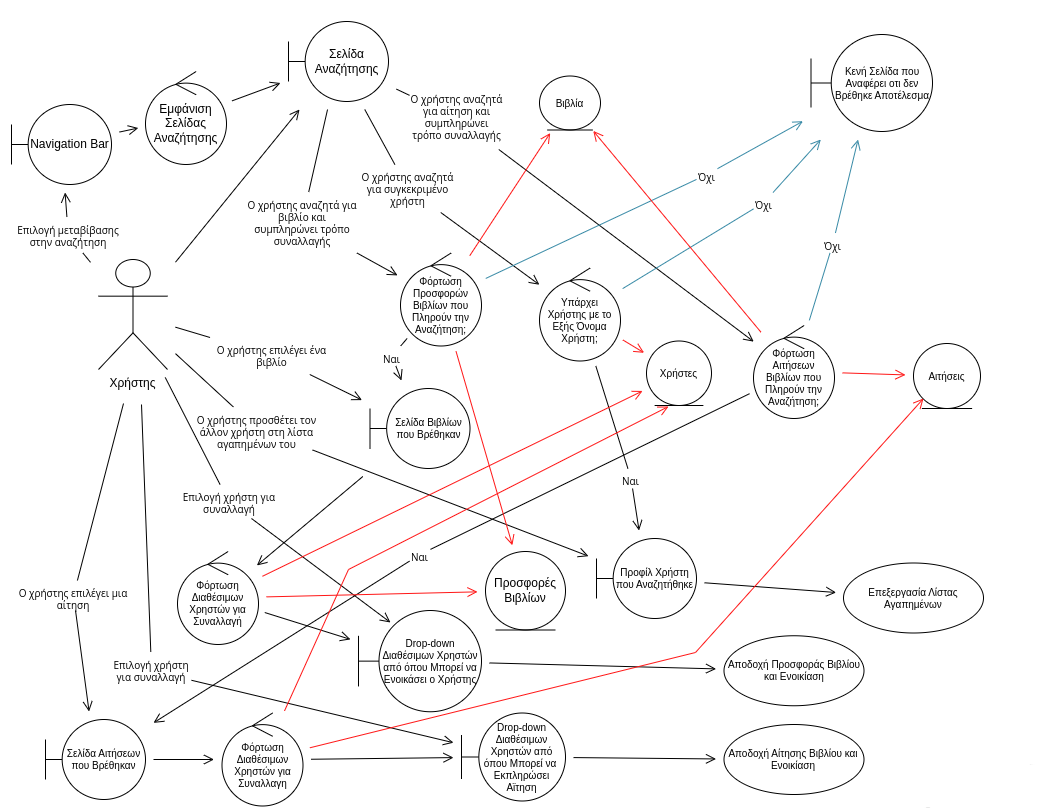
\includegraphics[width=\textwidth]{Search Robustness.png}
	\caption{Robustness Diagram: Αναζήτηση βιβλίων / χρήστη / αιτήσεων}
	\label{Robustness Diagram: Αναζήτηση βιβλίων / χρήστη / αιτήσεων}
\end{figure}
\label{Search}

Σχετικά με το robustness diagram για την "Αναζήτηση βιβλίων / χρήστη / αιτήσεων", θέλαμε να αναφέρουμε πως τα συνοριακά αντικείμενα "Σελίδα Αναζήτησης", "Σελίδα Αναζήτησης: Βιβλία που Βρέθηκαν", "Σελίδα Αναζήτησης: Διαθέσιμοι Χρήστες από όπου Μπορεί να Ενοικιάσει ο Χρήστης", "Σελίδα Αναζήτησης: Προφίλ Χρήστη που Αναζητήθηκε μαζί με τις αξιολογήσεις του", "Σελίδα Αναζήτησης: Αιτήσεις που Βρέθηκαν", "Σελίδα Αναζήτησης: Διαθέσιμοι Χρήστες για τους οποίους μπορεί να Εκπληρώσει Αίτηση" και "Σελίδα Αναζήτησης: Κενή Αναζήτηση" όλες αναφέρονται στην ίδια οθόνη της "Σελίδας Αναζήτησης".

Ο λόγος που χρησιμοποιούμε πολλά συνοριακά για την ίδια οθόνη είναι για να φαίνεται καθαρά η ακολουθία των ενεργειών στο διάγραμμα και να μην σπάσουμε το τεστ των ακμών, μέσω της επιστροφής σε προηγούμενο συνοριακό.

Για λόγους απλότητας όμως, μεταφέροντας τα συνοριακά αντικείμενα ως κλάσεις στα sequence diagrams και στο class diagram σε επόμενο βήμα, και τέλος και στο κώδικα, θα μεταφέρουμε μόνο τη "Σελίδα Αναζήτησης". Γνωρίζουμε ότι θα μπορούσαμε να δημιουργήσουμε περισσότερες κλάσεις για τα αποτελέσματα για παράδειγμα, αλλά πιστεύουμε ότι θα οδηγούσε σε πολύ σύνθετη αρχιτεκτονική κώδικα, καθώς και οι επιπλέον κλάσεις που θα δημιουργούσαμε δεν θα μπορούσαν να επαναχρησιμοποιηθούν αλλού. Οπότε προτιμήσαμε να θεωρήσουμε τη "Σελίδα Αναζήτησης (SearchPage κλάση αργότερα) ως μια κλάση μαζί με όλο της το περιεχόμενο.

\subsection{Αποδοχή Προσφοράς Βιβλίου και Ενοικίαση}
\begin{figure}[H]
	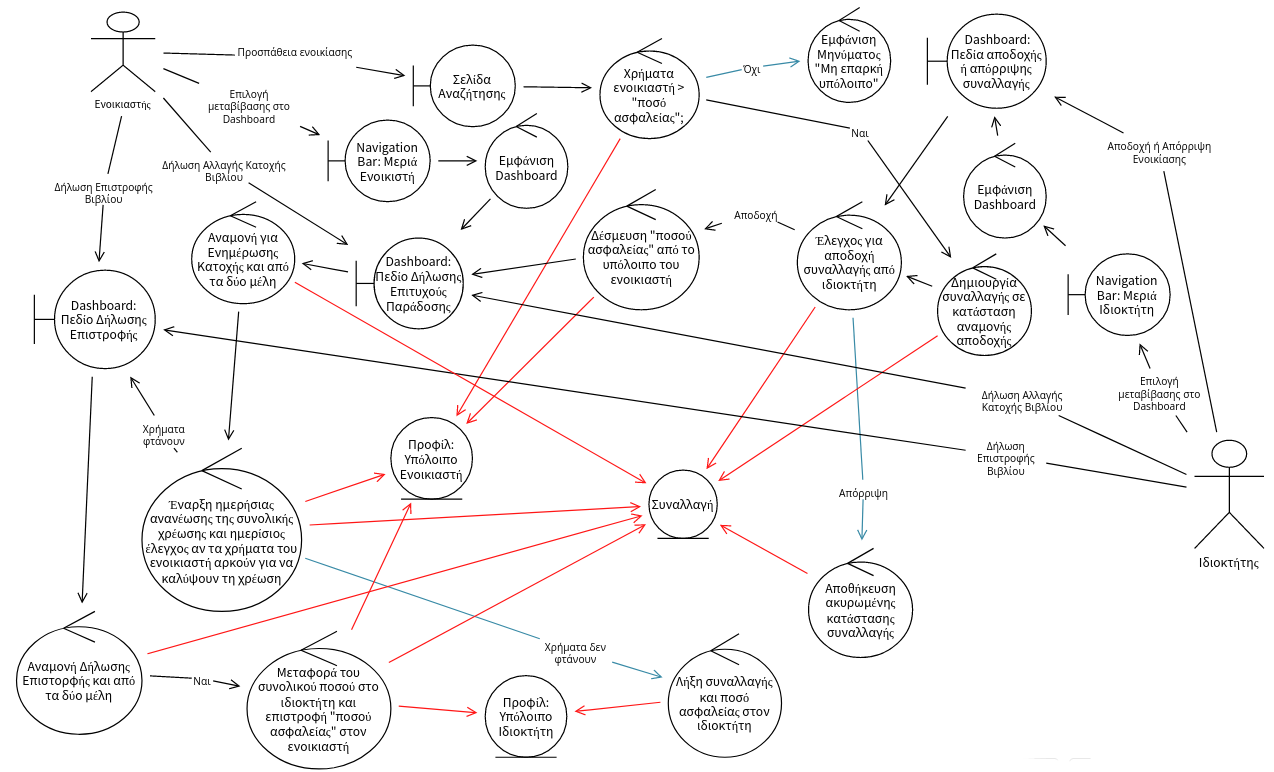
\includegraphics[width=\textwidth]{Accept Book Offer and Rent Robustness.png}
	\caption{Robustness Diagram: Αποδοχή Προσφοράς Βιβλίου και Ενοικίαση}
	\label{Robustness Diagram: Αποδοχή Προσφοράς Βιβλίου και Ενοικίαση}
\end{figure}
\label{Rent}

Στο robustness diagram για τη "Αποδοχή προσφοράς Βιβλίου και Ενοικίαση" έχουμε κάνει πάλι παρόμοια παραδοχή για ορισμένα συνοριακά αντικείμενα όπως κάναμε στο κεφάλαιο \ref{Search}, αυτή τη φορά όμως θεωρώντας τα συνοριακά αντικείμενα "Dashboard Πεδία αποδοχής ή απόρριψης συναλλαγής", "Dashboard: Πεδίο Δήλωσης Επιτυχούς Παράδοσης", "Dashboard: Πεδίο Δήλωσης Επιστροφής" να αναφέρονται σε διαφορετικά τμήματα της ίδιας οθόνης, του "Dashboard", που θα μεταφερθεί ως μια κλάση στο class diagram, sequence diagram και κώδικα.

Επίσης αναφέρουμε ότι τα συνοριακά αντικείμενα "Navigation Bar: Μεριά Ενοικιαστή" και "Navigation Bar: Μεριά Ιδιοκτήτη" αναφέρονται σε δύο διαφορετικά στιγμιότυπα της ίδιας κλάσης, ένα για κάθε χειριστή της εφαρμογής. Οπότε και αυτό μεταφέρεται σαν μια κλάση στο class diagram και robustness diagram και κώδικα (την GUI).

Τέλος τα αντικείμενα οντότητας "Προφίλ: Υπόλοιπο Ενοικιαστή" και "Προφίλ: Υπόλοιπο Ιδιοκτήτη" αναφέρονται πάλι σε δύο διαφορετικά στιγμιότυπα της μετέπειτα κλάσης που δημιουργήσαμε στο sequence diagram "User" (και μεταφέρθηκε στο class diagram και κώδικα), η οποία κλάση περιέχει πεδίο για υπόλοιπο χρήστη. Ο λόγος που και ο ενοικιαστής και ιδιοκτήτης είναι στιγμιότυπα της ίδιας κλάσης "User" είναι επειδή όλοι οι χρήστες μπορούν να είναι και ιδιοκτήτες και ενοικιαστές σε διαφορετικές συναλλαγές.

\subsection{Αποδοχή Αίτησης Βιβλίου και Ενοικίαση}
\begin{figure}[H]
	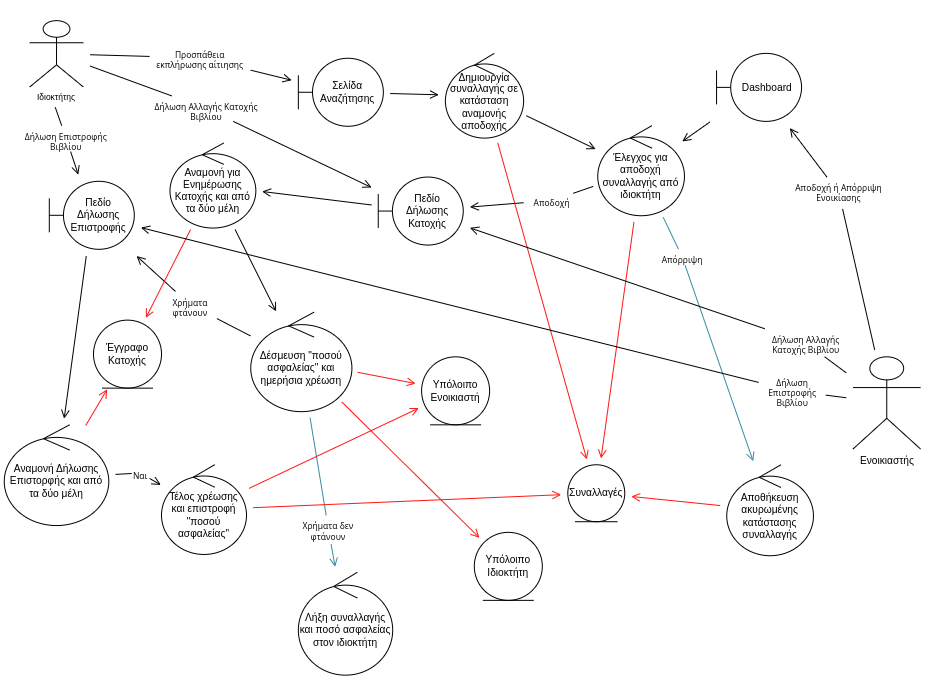
\includegraphics[width=\textwidth]{Accept Request Offer and Rent Robustness.png}
	\caption{Robustness Diagram: Αποδοχή Αίτησης Βιβλίου και Ενοικίαση}
	\label{Robustness Diagram: Αποδοχή Αίτησης Βιβλίου και Ενοικίαση}
\end{figure}

Στο robustness diagram για τη "Αποδοχή Αίτησης Βιβλίου και Ενοικίαση" ισχύουν οι ίδιες σημειώσεις και παραδοχές που ίσχυαν και για το robustness diagram στο κεφάλαιο \ref{Rent}, εφόσον τα δύο use cases "Αποδοχή Αίτησης Βιβλίου και Ενοικίαση" και "Αποδοχή Προσφοράς Βιβλίου και Ενοικίαση" αποτελούν δύο πτυχές της ίδιας διαδικασίας, που εξηγήσαμε στο τεχνικό κείμενο "Use-cases-v1.0" γιατί τα αναφέρουμε ξεχωριστά.

\subsection{Διαχείριση των βιβλίων που προσφέρει ο χρήστης προς ενοικίαση από άλλους}
\begin{figure}[H]
	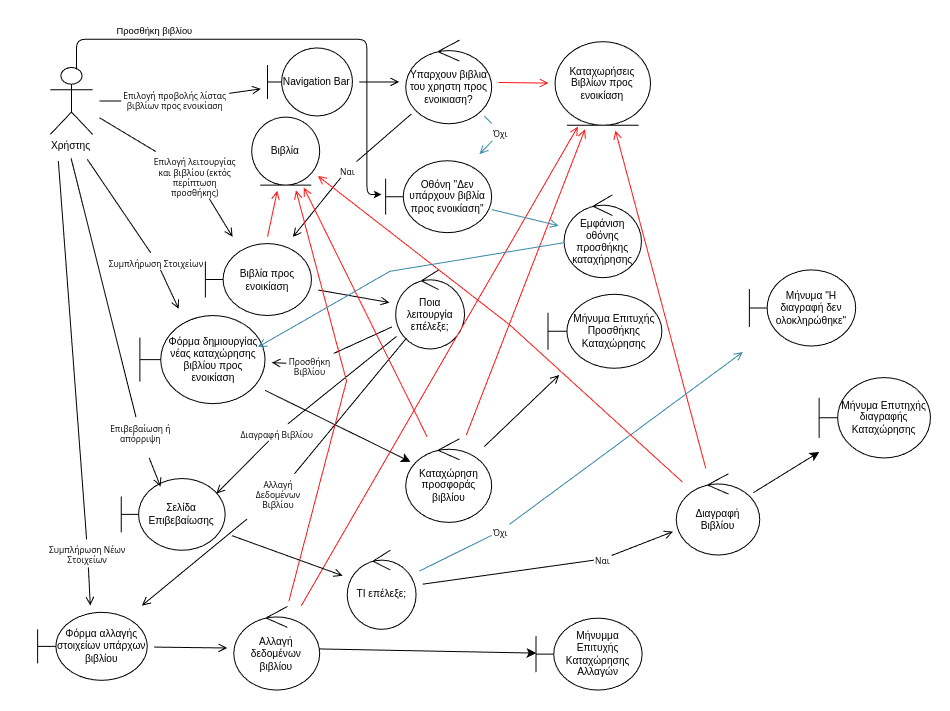
\includegraphics[width=\textwidth]{Manage User Book Listings Robustness.png}
	\caption{Robustness Diagram: Διαχείριση των βιβλίων που προσφέρει ο χρήστης προς ενοικίαση από άλλους}
	\label{Robustness Diagram: Διαχείριση των βιβλίων που προσφέρει ο χρήστης προς ενοικίαση από άλλους}
\end{figure}

Εδώ τα boundary objects "Βιβλία προς ενοικίαση", "Βιβλία προς ενοικίαση: Κενή οθόνη", "Βιβλία προς ενοικίαση: Φόρμα προσθήκης καταχώρησης", "Βιβλία προς ενοικίαση: Φόρμα αλλαγής τιμής και τύπου συναλλαγής" και "Βιβλία προς ενοικίαση: Ανανεωμένη σελίδα με τις αλλαγές" αναφέρονται όλες σε διαφορετικά μέρη ή σε διαφορετικές στιγμές της ίδιας σελίδας, οπότε τα μεταφέρουμε σαν μια κλάση στο sequence diagram, στο class diagram και στον κώδικα.

\subsection{Διαχείριση των αιτήσεων που έχει κάνει ο χρήστης}
\begin{figure}[H]
	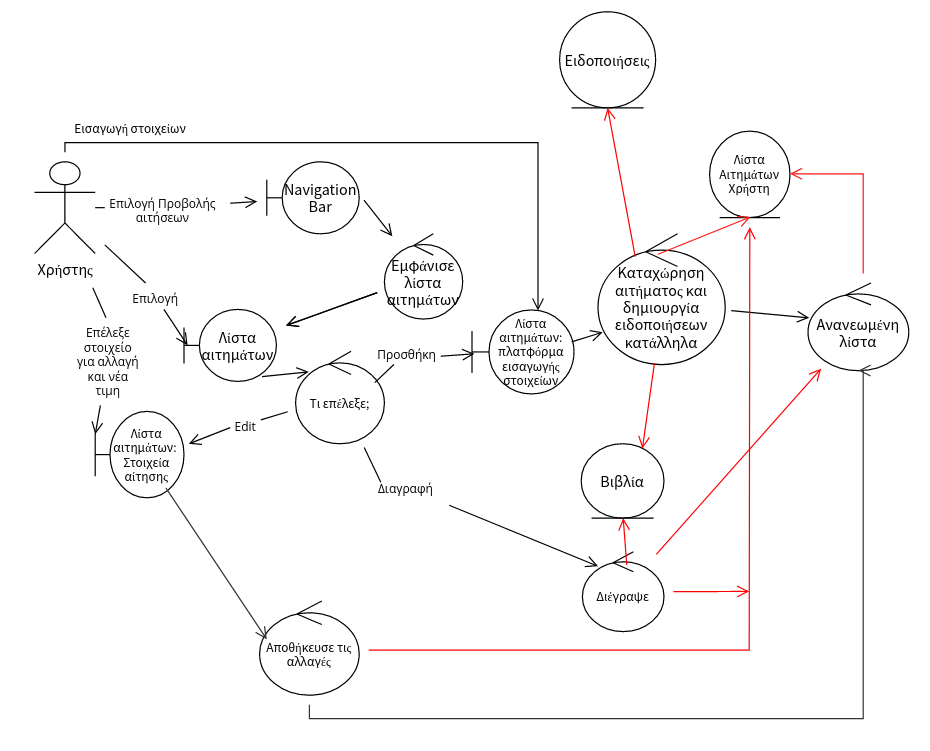
\includegraphics[width=\textwidth]{Manage User Requests Robustness.png}
	\caption{Robustness Diagram: Διαχείριση των αιτήσεων που έχει κάνει ο χρήστης}
	\label{Robustness Diagram: Διαχείριση των αιτήσεων που έχει κάνει ο χρήστης}
\end{figure}

Εδώ τα boundary objects "Λίστα αιτημάτων", "Λίστα αιτημάτων: Στοιχεία αίτησης" και "Λίστα αιτημάτων: πλατφόρμα εισαγωγής στοιχείων" αναφέρονται όλες σε διαφορετικά μέρη ή σε διαφορετικές στιγμές της ίδιας σελίδας, οπότε τα μεταφέρουμε σαν μια κλάση στο sequence diagram, στο class diagram και στον κώδικα.

\subsection{Αξιολόγηση άλλων χρηστών μετά από την ολοκλήρωση συναλλαγής}
\begin{figure}[H]
	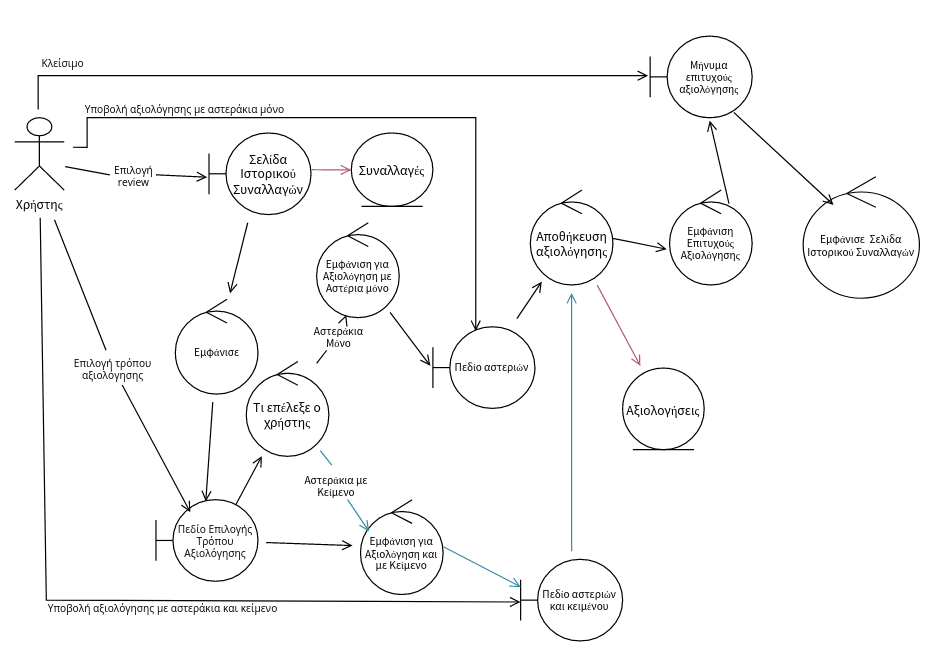
\includegraphics[width=\textwidth]{Review after Transaction Robustness.png}
	\caption{Robustness Diagram: Αξιολόγηση άλλων χρηστών μετά από την ολοκλήρωση συναλλαγής}
	\label{Robustness Diagram: Αξιολόγηση άλλων χρηστών μετά από την ολοκλήρωση συναλλαγής}
\end{figure}

Εδώ τα boundary objects "Σελίδα Αξιολόγησης", "Σελίδα Αξιολόγησης: Πεδίο αστεριών" και "Σελίδα Αξιολόγησης: Πεδίο αστεριών και κειμένου" αναφέρονται όλες σε διαφορετικά μέρη ή σε διαφορετικές στιγμές της ίδιας σελίδας, οπότε τα μεταφέρουμε σαν μια κλάση στο sequence diagram, στο class diagram και στον κώδικα.

\subsection{Προβολή και Επεξεργασία στοιχείων λογαριασμού χρήστη}
\textbf{Σημείωση:} Στο διάγραμμα αυτό τα δύο boundary objects "Οθόνη Προφίλ με Δυνατότητα Επεξεργασίας" και "Οθόνη προφίλ με ανανεωμένα στοιχεία" αναφέρονται στην ίδια οθόνη, πριν και μετά την αλλαγή αντίστοιχα. Ο λόγος που τα βάλαμε ξεχωριστά είναι για να φαίνεται η αλληλουχία των πράξεων.
\begin{figure}[H]
	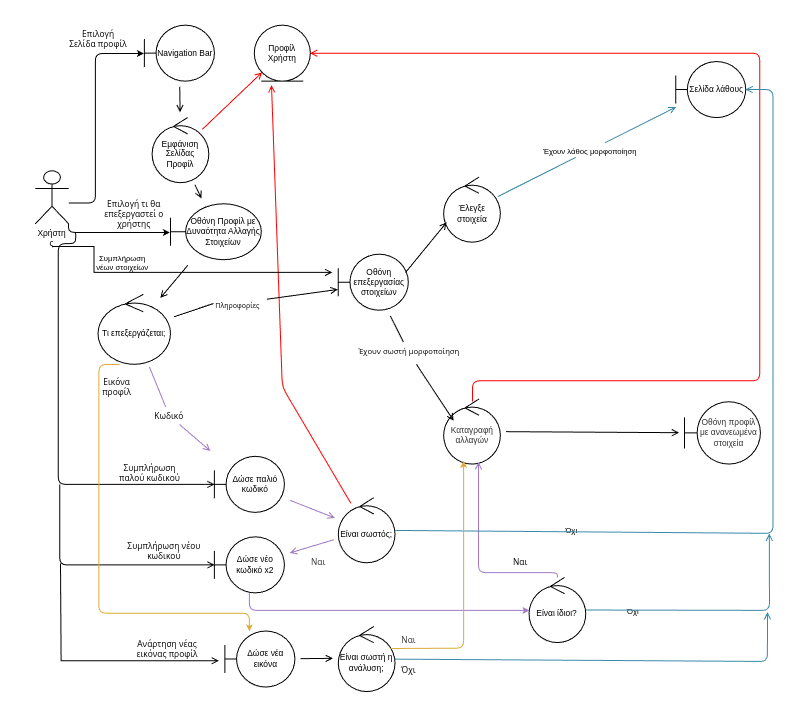
\includegraphics[width=\textwidth]{View and Edit User Account Details Robustness.png}
	\caption{Robustness Diagram: Προβολή και Επεξεργασία στοιχείων λογαριασμού χρήστη}
	\label{Robustness Diagram: Προβολή και Επεξεργασία στοιχείων λογαριασμού χρήστη}
\end{figure}

Εδώ τα boundary objects "Οθόνη Προφίλ: Στοιχεία με δυνατότητα επεξεργασίας", "Οθόνη Προφίλ: Πεδία επεξεργασίας στοιχείων", "Οθόνη Προφίλ: Πεδίο παλιού κωδικού", "Οθόνη Προφίλ: Πεδία νέου κωδικού", "Οθόνη Προφίλ: Pop-up σφάλματος" και "Οθόνη Προφίλ: Εμφάνιση ανανεωμένων στοιχείων" αναφέρονται όλες σε διαφορετικά μέρη ή σε διαφορετικές στιγμές της ίδιας σελίδας, οπότε τα μεταφέρουμε σαν μια κλάση στο sequence diagram, στο class diagram και στον κώδικα.

\subsection{Επεξεργασία χρηματικού υπολοίπου χρήστη}
\begin{figure}[H]
	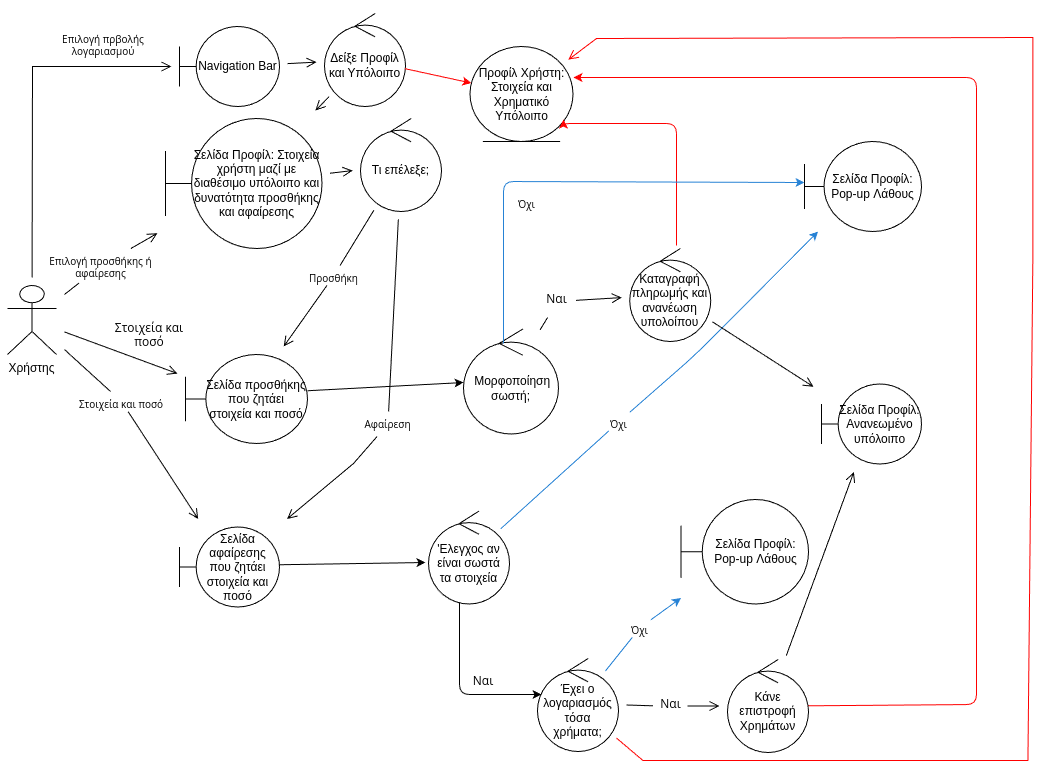
\includegraphics[width=\textwidth]{Edit User Balance Robustness.png}
	\caption{Robustness Diagram: Επεξεργασία χρηματικού υπολοίπου χρήστη}
	\label{Robustness Diagram: Επεξεργασία χρηματικού υπολοίπου χρήστη}
\end{figure}

Εδώ τα boundary objects "Σελίδα Προφίλ: Στοιχεία χρήστη μαζί με διαθέσιμο υπόλοιπο και δυνατότητα προσθήκης και αφαίρεσης", "Σελίδα Προφίλ: Επιλογή προσθήκης με πεδίο ποσού", "Σελίδα Προφίλ: Επιλογή αφαίρεσης με πεδίο ποσού", "Σελίδα Προφίλ: Pop-up λάθους" και "Σελίδα Προφίλ: Ανανεωμένο υπόλοιπο" αναφέρονται όλες σε διαφορετικά μέρη ή σε διαφορετικές στιγμές της ίδιας σελίδας, οπότε τα μεταφέρουμε σαν μια κλάση στο sequence diagram, στο class diagram και στον κώδικα.

\subsection{Επεξεργασία λίστας αγαπημένων και χρήση συστήματος ειδοποιήσεων}
\begin{figure}[H]
	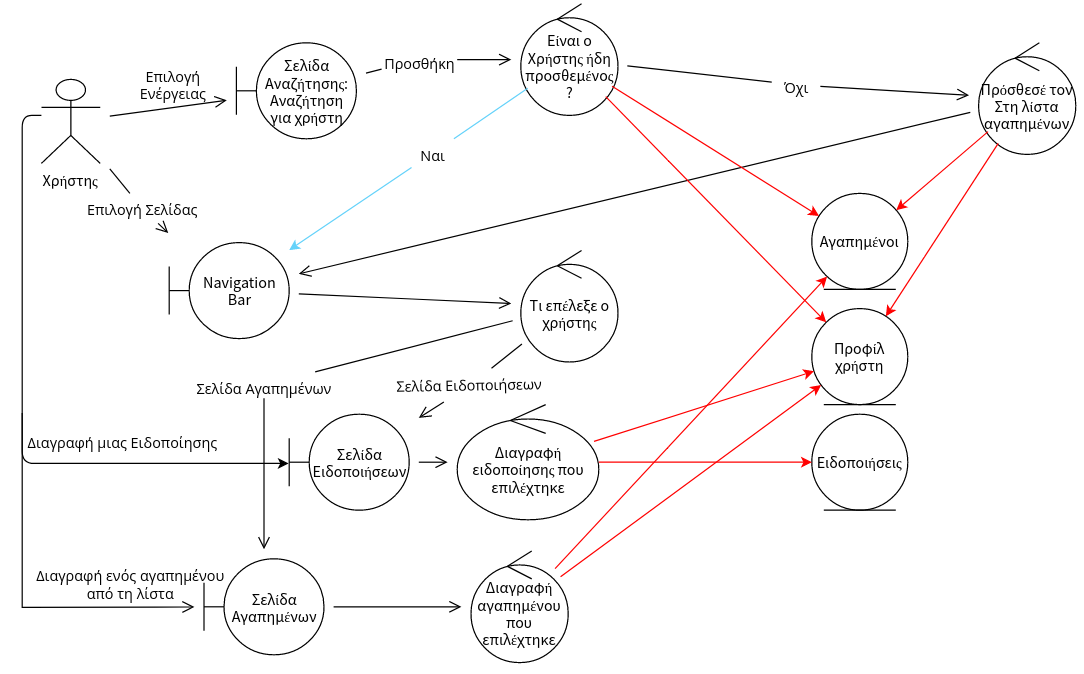
\includegraphics[width=\textwidth]{Favorite Users and Notification System Robustness.png}
	\caption{Robustness Diagram: Επεξεργασία λίστας αγαπημένων και χρήση συστήματος ειδοποιήσεων}
	\label{Robustness Diagram: Επεξεργασία λίστας αγαπημένων και χρήση συστήματος ειδοποιήσεων}
\end{figure}

\subsection{Προβολή ιστορικού συναλλαγών και στατιστικών}
\begin{figure}[H]
	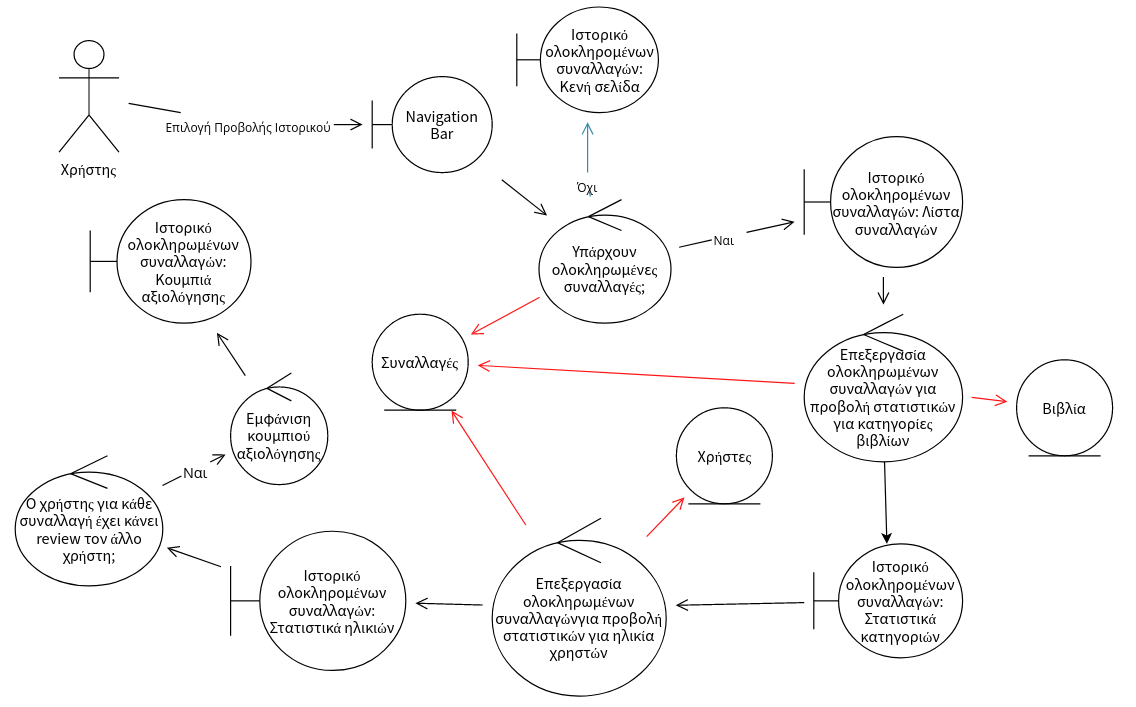
\includegraphics[width=\textwidth]{History and Statistics Robustness.png}
	\caption{Robustness Diagram: Προβολή ιστορικού συναλλαγών και στατιστικών}
	\label{Robustness Diagram: Προβολή ιστορικού συναλλαγών και στατιστικών}
\end{figure}

Εδώ τα boundary objects "Ιστορικό ολοκληρωμένων συναλλαγών: Κενή σελίδα", "Ιστορικό ολοκληρωμένων συναλλαγών: Λίστα συναλλαγών", "Ιστορικό ολοκληρωμένων συναλλαγών: Στατιστικά κατηγοριών", "Ιστορικό ολοκληρωμένων συναλλαγών: Στατιστικά ηλικιών" και "Ιστορικό ολοκληρωμένων συναλλαγών: Κουμπιά αξιολόγησης" αναφέρονται όλες σε διαφορετικά μέρη ή σε διαφορετικές στιγμές της ίδιας σελίδας, οπότε τα μεταφέρουμε σαν μια κλάση στο sequence diagram, στο class diagram και στον κώδικα.

\section{Συμμετοχή και Ρόλοι στη Συγγραφή του Κειμένου}
\begin{enumerate}
	\item \textbf{Γρηγόρης Καπαδούκας:} Author (Κεφαλαίων 1.1, 1.2, 1.3), Editor Όλων, Reviewer Όλων
	\item \textbf{Χρήστος Μπεστητζάνος:} Author (Κεφαλαίων 1.5, 1.6)
   	\item \textbf{Νικόλαος Αυγέρης:} Author (Κεφαλαίων 1.7, 1.8, 1.9)
	\item \textbf{Περικλής Κοροντζής:} Author (Κεφαλαίων 1.4, 1.10)
\end{enumerate}

\section{Αλλαγές από έκδοση σε έκδοση}

\subsection{Από έκδοση v0.1 σε έκδοση v0.2}
\begin{itemize}
    \item Αλλαγή στο Robustness Diagram για "Αναζήτηση βιβλίων / χρήστη / αιτήσεων".
    \item Διαγραφή των Robustness Diagrams για "Αναζήτηση βιβλίων / χρήστη / αιτήσεων" και "Ενοικίαση βιβλίου από άλλο χρήστη" και αντικατάστασή τους με τα αντίστοιχα για "Αποδοχή Προσφοράς Βιβλίου και Ενοικίαση" και "Αποδοχή Αίτησης Βιβλίου και Ενοικίαση".
    \item Ανανέωση του Robustness Diagram για "Επεξεργασία χρηματικού υπολοίπου χρήστη".
    \item Ανανέωση του Robustness Diagram για "Επεξεργασία λίστας αγαπημένων και χρήση συστήματος ειδοποιήσεων".
    \item Ανανέωση του Robustness Diagram για "Προβολή και Επεξεργασία στοιχείων λογαριασμού χρήστη".
    \item Ανανέωση του Robustness Diagram για "Διαχείριση των βιβλίων που προσφέρει ο χρήστης
προς ενοικίαση από άλλους".
    \item Διόρθωση λάθος αρίθμησης κεφαλαίων στο Κεφάλαιο 2.
\end{itemize}

\subsection{Από έκδοση v0.2 σε έκδοση v1.0}
\begin{itemize}
    \item Διόρθωση όλων των Robustness Diagrams, ώστε να εξηγήσουμε καλύτερα ποια boundary objects τελικά αναφέρονται τις ίδιες οθόνες (και κλάσεις) και ποια entity objects αναφέρονται πάλι την ίδια βασική κλάση.
    \item Επίσης ό,τι αλλαγές έγιναν στη πορεία φαίνονται στα ανανεωμένα Robustness Diagrams
\end{itemize}

\end{document}
